% Options for packages loaded elsewhere
\PassOptionsToPackage{unicode}{hyperref}
\PassOptionsToPackage{hyphens}{url}
\PassOptionsToPackage{dvipsnames,svgnames,x11names}{xcolor}
%
\documentclass[
  letterpaper,
  DIV=11,
  numbers=noendperiod]{scrreprt}

\usepackage{amsmath,amssymb}
\usepackage{iftex}
\ifPDFTeX
  \usepackage[T1]{fontenc}
  \usepackage[utf8]{inputenc}
  \usepackage{textcomp} % provide euro and other symbols
\else % if luatex or xetex
  \usepackage{unicode-math}
  \defaultfontfeatures{Scale=MatchLowercase}
  \defaultfontfeatures[\rmfamily]{Ligatures=TeX,Scale=1}
\fi
\usepackage{lmodern}
\ifPDFTeX\else  
    % xetex/luatex font selection
\fi
% Use upquote if available, for straight quotes in verbatim environments
\IfFileExists{upquote.sty}{\usepackage{upquote}}{}
\IfFileExists{microtype.sty}{% use microtype if available
  \usepackage[]{microtype}
  \UseMicrotypeSet[protrusion]{basicmath} % disable protrusion for tt fonts
}{}
\makeatletter
\@ifundefined{KOMAClassName}{% if non-KOMA class
  \IfFileExists{parskip.sty}{%
    \usepackage{parskip}
  }{% else
    \setlength{\parindent}{0pt}
    \setlength{\parskip}{6pt plus 2pt minus 1pt}}
}{% if KOMA class
  \KOMAoptions{parskip=half}}
\makeatother
\usepackage{xcolor}
\setlength{\emergencystretch}{3em} % prevent overfull lines
\setcounter{secnumdepth}{5}
% Make \paragraph and \subparagraph free-standing
\ifx\paragraph\undefined\else
  \let\oldparagraph\paragraph
  \renewcommand{\paragraph}[1]{\oldparagraph{#1}\mbox{}}
\fi
\ifx\subparagraph\undefined\else
  \let\oldsubparagraph\subparagraph
  \renewcommand{\subparagraph}[1]{\oldsubparagraph{#1}\mbox{}}
\fi

\usepackage{color}
\usepackage{fancyvrb}
\newcommand{\VerbBar}{|}
\newcommand{\VERB}{\Verb[commandchars=\\\{\}]}
\DefineVerbatimEnvironment{Highlighting}{Verbatim}{commandchars=\\\{\}}
% Add ',fontsize=\small' for more characters per line
\usepackage{framed}
\definecolor{shadecolor}{RGB}{241,243,245}
\newenvironment{Shaded}{\begin{snugshade}}{\end{snugshade}}
\newcommand{\AlertTok}[1]{\textcolor[rgb]{0.68,0.00,0.00}{#1}}
\newcommand{\AnnotationTok}[1]{\textcolor[rgb]{0.37,0.37,0.37}{#1}}
\newcommand{\AttributeTok}[1]{\textcolor[rgb]{0.40,0.45,0.13}{#1}}
\newcommand{\BaseNTok}[1]{\textcolor[rgb]{0.68,0.00,0.00}{#1}}
\newcommand{\BuiltInTok}[1]{\textcolor[rgb]{0.00,0.23,0.31}{#1}}
\newcommand{\CharTok}[1]{\textcolor[rgb]{0.13,0.47,0.30}{#1}}
\newcommand{\CommentTok}[1]{\textcolor[rgb]{0.37,0.37,0.37}{#1}}
\newcommand{\CommentVarTok}[1]{\textcolor[rgb]{0.37,0.37,0.37}{\textit{#1}}}
\newcommand{\ConstantTok}[1]{\textcolor[rgb]{0.56,0.35,0.01}{#1}}
\newcommand{\ControlFlowTok}[1]{\textcolor[rgb]{0.00,0.23,0.31}{#1}}
\newcommand{\DataTypeTok}[1]{\textcolor[rgb]{0.68,0.00,0.00}{#1}}
\newcommand{\DecValTok}[1]{\textcolor[rgb]{0.68,0.00,0.00}{#1}}
\newcommand{\DocumentationTok}[1]{\textcolor[rgb]{0.37,0.37,0.37}{\textit{#1}}}
\newcommand{\ErrorTok}[1]{\textcolor[rgb]{0.68,0.00,0.00}{#1}}
\newcommand{\ExtensionTok}[1]{\textcolor[rgb]{0.00,0.23,0.31}{#1}}
\newcommand{\FloatTok}[1]{\textcolor[rgb]{0.68,0.00,0.00}{#1}}
\newcommand{\FunctionTok}[1]{\textcolor[rgb]{0.28,0.35,0.67}{#1}}
\newcommand{\ImportTok}[1]{\textcolor[rgb]{0.00,0.46,0.62}{#1}}
\newcommand{\InformationTok}[1]{\textcolor[rgb]{0.37,0.37,0.37}{#1}}
\newcommand{\KeywordTok}[1]{\textcolor[rgb]{0.00,0.23,0.31}{#1}}
\newcommand{\NormalTok}[1]{\textcolor[rgb]{0.00,0.23,0.31}{#1}}
\newcommand{\OperatorTok}[1]{\textcolor[rgb]{0.37,0.37,0.37}{#1}}
\newcommand{\OtherTok}[1]{\textcolor[rgb]{0.00,0.23,0.31}{#1}}
\newcommand{\PreprocessorTok}[1]{\textcolor[rgb]{0.68,0.00,0.00}{#1}}
\newcommand{\RegionMarkerTok}[1]{\textcolor[rgb]{0.00,0.23,0.31}{#1}}
\newcommand{\SpecialCharTok}[1]{\textcolor[rgb]{0.37,0.37,0.37}{#1}}
\newcommand{\SpecialStringTok}[1]{\textcolor[rgb]{0.13,0.47,0.30}{#1}}
\newcommand{\StringTok}[1]{\textcolor[rgb]{0.13,0.47,0.30}{#1}}
\newcommand{\VariableTok}[1]{\textcolor[rgb]{0.07,0.07,0.07}{#1}}
\newcommand{\VerbatimStringTok}[1]{\textcolor[rgb]{0.13,0.47,0.30}{#1}}
\newcommand{\WarningTok}[1]{\textcolor[rgb]{0.37,0.37,0.37}{\textit{#1}}}

\providecommand{\tightlist}{%
  \setlength{\itemsep}{0pt}\setlength{\parskip}{0pt}}\usepackage{longtable,booktabs,array}
\usepackage{calc} % for calculating minipage widths
% Correct order of tables after \paragraph or \subparagraph
\usepackage{etoolbox}
\makeatletter
\patchcmd\longtable{\par}{\if@noskipsec\mbox{}\fi\par}{}{}
\makeatother
% Allow footnotes in longtable head/foot
\IfFileExists{footnotehyper.sty}{\usepackage{footnotehyper}}{\usepackage{footnote}}
\makesavenoteenv{longtable}
\usepackage{graphicx}
\makeatletter
\def\maxwidth{\ifdim\Gin@nat@width>\linewidth\linewidth\else\Gin@nat@width\fi}
\def\maxheight{\ifdim\Gin@nat@height>\textheight\textheight\else\Gin@nat@height\fi}
\makeatother
% Scale images if necessary, so that they will not overflow the page
% margins by default, and it is still possible to overwrite the defaults
% using explicit options in \includegraphics[width, height, ...]{}
\setkeys{Gin}{width=\maxwidth,height=\maxheight,keepaspectratio}
% Set default figure placement to htbp
\makeatletter
\def\fps@figure{htbp}
\makeatother
\newlength{\cslhangindent}
\setlength{\cslhangindent}{1.5em}
\newlength{\csllabelwidth}
\setlength{\csllabelwidth}{3em}
\newlength{\cslentryspacingunit} % times entry-spacing
\setlength{\cslentryspacingunit}{\parskip}
\newenvironment{CSLReferences}[2] % #1 hanging-ident, #2 entry spacing
 {% don't indent paragraphs
  \setlength{\parindent}{0pt}
  % turn on hanging indent if param 1 is 1
  \ifodd #1
  \let\oldpar\par
  \def\par{\hangindent=\cslhangindent\oldpar}
  \fi
  % set entry spacing
  \setlength{\parskip}{#2\cslentryspacingunit}
 }%
 {}
\usepackage{calc}
\newcommand{\CSLBlock}[1]{#1\hfill\break}
\newcommand{\CSLLeftMargin}[1]{\parbox[t]{\csllabelwidth}{#1}}
\newcommand{\CSLRightInline}[1]{\parbox[t]{\linewidth - \csllabelwidth}{#1}\break}
\newcommand{\CSLIndent}[1]{\hspace{\cslhangindent}#1}

\KOMAoption{captions}{tableheading}
\makeatletter
\makeatother
\makeatletter
\@ifpackageloaded{bookmark}{}{\usepackage{bookmark}}
\makeatother
\makeatletter
\@ifpackageloaded{caption}{}{\usepackage{caption}}
\AtBeginDocument{%
\ifdefined\contentsname
  \renewcommand*\contentsname{Table of contents}
\else
  \newcommand\contentsname{Table of contents}
\fi
\ifdefined\listfigurename
  \renewcommand*\listfigurename{List of Figures}
\else
  \newcommand\listfigurename{List of Figures}
\fi
\ifdefined\listtablename
  \renewcommand*\listtablename{List of Tables}
\else
  \newcommand\listtablename{List of Tables}
\fi
\ifdefined\figurename
  \renewcommand*\figurename{Figure}
\else
  \newcommand\figurename{Figure}
\fi
\ifdefined\tablename
  \renewcommand*\tablename{Table}
\else
  \newcommand\tablename{Table}
\fi
}
\@ifpackageloaded{float}{}{\usepackage{float}}
\floatstyle{ruled}
\@ifundefined{c@chapter}{\newfloat{codelisting}{h}{lop}}{\newfloat{codelisting}{h}{lop}[chapter]}
\floatname{codelisting}{Listing}
\newcommand*\listoflistings{\listof{codelisting}{List of Listings}}
\makeatother
\makeatletter
\@ifpackageloaded{caption}{}{\usepackage{caption}}
\@ifpackageloaded{subcaption}{}{\usepackage{subcaption}}
\makeatother
\makeatletter
\@ifpackageloaded{tcolorbox}{}{\usepackage[skins,breakable]{tcolorbox}}
\makeatother
\makeatletter
\@ifundefined{shadecolor}{\definecolor{shadecolor}{rgb}{.97, .97, .97}}
\makeatother
\makeatletter
\makeatother
\makeatletter
\makeatother
\ifLuaTeX
  \usepackage{selnolig}  % disable illegal ligatures
\fi
\IfFileExists{bookmark.sty}{\usepackage{bookmark}}{\usepackage{hyperref}}
\IfFileExists{xurl.sty}{\usepackage{xurl}}{} % add URL line breaks if available
\urlstyle{same} % disable monospaced font for URLs
\hypersetup{
  pdftitle={learning diary},
  pdfauthor={Zhongzhen Ouyang},
  colorlinks=true,
  linkcolor={blue},
  filecolor={Maroon},
  citecolor={Blue},
  urlcolor={Blue},
  pdfcreator={LaTeX via pandoc}}

\title{learning diary}
\author{Zhongzhen Ouyang}
\date{2024-02-01}

\begin{document}
\maketitle
\ifdefined\Shaded\renewenvironment{Shaded}{\begin{tcolorbox}[borderline west={3pt}{0pt}{shadecolor}, interior hidden, enhanced, breakable, boxrule=0pt, sharp corners, frame hidden]}{\end{tcolorbox}}\fi

\renewcommand*\contentsname{Table of contents}
{
\hypersetup{linkcolor=}
\setcounter{tocdepth}{2}
\tableofcontents
}
\bookmarksetup{startatroot}

\hypertarget{introduction}{%
\chapter{Introduction}\label{introduction}}

This is the introduction to my document.

\bookmarksetup{startatroot}

\hypertarget{week1}{%
\chapter{Week1}\label{week1}}

\bookmarksetup{startatroot}

\hypertarget{week6}{%
\chapter{Week6}\label{week6}}

\bookmarksetup{startatroot}

\hypertarget{introduction-1}{%
\chapter{Introduction}\label{introduction-1}}

This is a book created from markdown and executable code.

See Knuth (1984) for additional discussion of literate programming.

\bookmarksetup{startatroot}

\hypertarget{week-1---introduction-to-remote-sensing}{%
\chapter{Week 1 - Introduction to Remote
Sensing}\label{week-1---introduction-to-remote-sensing}}

\hypertarget{summary}{%
\subsection{Summary}\label{summary}}

\begin{itemize}
\tightlist
\item
  Remote sensing is defined as acquiring information from a distance.
  Remote sensing can collect data without physical contact with objects
  by sensors.
\item
  Passive or active sensors. Active sensors have an energy source and
  will actively emit electromagnetic energy and then receive
\item
  Electromagnetic energy

  \begin{enumerate}
  \def\labelenumi{\arabic{enumi}.}
  \tightlist
  \item
    Wavelength: long wavelength = low frequency = low energy
  \item
    Electromagnetic spectrum: total range of wavelengths of EM radiant
  \item
    Energy interaction: reflected, absorbed by the surface, transmitted
    through the surface, scattered by particles in the atmosphere.
  \item
    Blue light shorter wavelength and more easily
    scatters(450nm-blue(shortest visible light) 550nm-green
    700nm-red(longest)).
  \item
    The spectral reflectance characteristics of surface materials are
    different. That is why sensors can identify materials. In the
    visible spectrum, chlorophyll in plant leaves strongly absorbs light
    in the blue and red regions, but reflects green light. This is why
    healthy vegetation appears green to our eyes.
  \item
    The sun is the primary source of EM energy
  \end{enumerate}
\item
  Four resolutions

  \begin{enumerate}
  \def\labelenumi{\arabic{enumi}.}
  \tightlist
  \item
    Spatial resolution the size of the raster grid per pixel
  \item
    Spectral resolution the number of bands sensor records data
  \item
    Radiometric resolution identify differences in light or reflectance,
    in practice this is the range of possible values.
  \item
    Temporal resolution the time it revisits
  \end{enumerate}
\end{itemize}

\hypertarget{application}{%
\subsection{Application}\label{application}}

\hypertarget{sentinel-2}{%
\subsubsection{Sentinel-2}\label{sentinel-2}}

\begin{enumerate}
\def\labelenumi{\arabic{enumi}.}
\tightlist
\item
  Spatial resolution of 10 m, 20 m and 60 m
\item
  Revisiting every 10 days
\item
  Multi-spectral data with 13 bands in the visible, near-infrared, and
  short-wave infrared part of the spectrum
\end{enumerate}

\begin{itemize}
\tightlist
\item
  Application
\end{itemize}

\begin{enumerate}
\def\labelenumi{\arabic{enumi}.}
\tightlist
\item
  Monitoring inland water bodies.
\end{enumerate}

\begin{enumerate}
\def\labelenumi{\arabic{enumi}.}
\setcounter{enumi}{1}
\tightlist
\item
  Watching coastal waters.
\end{enumerate}

\hypertarget{landset}{%
\subsubsection{Landset}\label{landset}}

The below figures are my practical output

green rectangle = bare earth pink rectangle = vegetation purple
rectangle = urban area red rectangle = water

It seems that the 7 bands.tif file is too large for my computer. I only
export GeoTIFFS with bands 2,3,4.

spectral profiles density plot

\hypertarget{reflection}{%
\subsection{reflection}\label{reflection}}

This is the very beginning of remote sensing, for me, it is the first
contact for me with the subject. Almost everything is new for me. The
only thing that I am familiar with is electromagnetic waves. Different
wavelength gives electromagnetic waves different properties, like the
penetrative ability. I thought longer wavelengths were easier to
penetrate, while shorter wavelengths were more difficult. However,
longer wavelengths of electromagnetic radiation, such as infrared and
microwaves, tend to penetrate certain substances more easily. This is
because some materials have lower absorption rates for longer
wavelengths, allowing radiation of these wavelengths to penetrate
relatively easily.

For other substances and specific wavelength ranges, the situation may
be different. For example, some materials have high absorption rates for
certain wavelengths of electromagnetic radiation, making it difficult
for radiation of these wavelengths to penetrate the material. This is
common in the visible light range, as many substances have high
absorption rates for visible light, making it difficult for visible
light to penetrate them. That is how the sensor identifies different
materials. Also, remote sensing sensors can capture electromagnetic
signals reflected or emitted from the Earth's surface and divide them
into multiple different bands. For example, a sensor for visible light
and infrared might be divided into several different bands, each
corresponding to a specific part of the visible light or infrared
spectrum. Different bands capture information about different types of
features on the Earth's surface, so the choice of bands is crucial for
the success of specific applications. That's why when I do practicals
there are so many bands that make me confused initially.

Another question I met that could take much time for me to figure out is
what are the differences between satellites. I know they have different
resolutions and bands, but what do the differences refer to, what
advantages do they have, and Why are so many types of satellites needed?

\bookmarksetup{startatroot}

\hypertarget{week-3---remote-sensing-data}{%
\chapter{Week 3 - Remote sensing
data}\label{week-3---remote-sensing-data}}

\hypertarget{summary-1}{%
\section{Summary}\label{summary-1}}

\hypertarget{corrections}{%
\subsection{Corrections}\label{corrections}}

\hypertarget{geometric}{%
\subsubsection{Geometric}\label{geometric}}

\begin{itemize}
\tightlist
\item
  Four reasons make image distortions:
\end{itemize}

\begin{enumerate}
\def\labelenumi{\arabic{enumi}.}
\tightlist
\item
  View angle
\item
  Topography
\item
  Wind
\item
  Rotation of the earth (from satellite)
\end{enumerate}

\begin{itemize}
\tightlist
\item
  Solution:
\end{itemize}

\begin{enumerate}
\def\labelenumi{\arabic{enumi}.}
\tightlist
\item
  several algorithms(linear regression, Helmert
  transformation,Polynomial algorithms 1-3, Thin Plate Spline (TPS),
  Projective transformation)
\item
  decide which model to be used(The model with the lowest RMSE will fit
  best)
\item
  re-sample the final raster
\end{enumerate}

\hypertarget{atmospheric}{%
\subsubsection{Atmospheric}\label{atmospheric}}

\begin{itemize}
\tightlist
\item
  Sources:
\end{itemize}

\begin{enumerate}
\def\labelenumi{\arabic{enumi}.}
\tightlist
\item
  Atmospheric scattering
\item
  Topographic attenuation
\end{enumerate}

\begin{itemize}
\tightlist
\item
  Method:
\end{itemize}

\begin{enumerate}
\def\labelenumi{\arabic{enumi}.}
\tightlist
\item
  Empirical Methods
\item
  Dark Object Subtraction
\item
  Psuedo-invariant Features (PIFs)
\item
  Atmospheric radiative transfer models
\end{enumerate}

\hypertarget{orthorectification-topographic-correction}{%
\subsubsection{Orthorectification / Topographic
correction}\label{orthorectification-topographic-correction}}

\begin{enumerate}
\def\labelenumi{\arabic{enumi}.}
\tightlist
\item
  Cosine correction
\item
  Minnaert correction
\item
  Statistical Empirical correction
\item
  C Correction (advancing the Cosine)
\end{enumerate}

\hypertarget{radiometric-calibration}{%
\subsubsection{Radiometric Calibration}\label{radiometric-calibration}}

\begin{enumerate}
\def\labelenumi{\arabic{enumi}.}
\tightlist
\item
  Radiometric Calibration = Digital Number to spectral radiance(true
  spectral radiance on earth surfaces is different with spectral
  radiance that sensors capture)
\item
  Sensor calibration: We use measurements to adjust
\item
  Reflectance: A ratio comparing the quantity of light emitted by a
  target to the quantity of light incident upon it.
\end{enumerate}

\begin{itemize}
\tightlist
\item
  should be considered in radiance correction
\end{itemize}

\hypertarget{joining-data-setsenhancements}{%
\subsection{Joining data
sets/Enhancements}\label{joining-data-setsenhancements}}

\hypertarget{joining-data-sets}{%
\subsubsection{Joining data sets}\label{joining-data-sets}}

\begin{itemize}
\tightlist
\item
  If one image is not sufficient to cover the area we wish to study, we
  need to merge several images.
\item
  is called `Mosaicking' in remote sensing
\item
  feather images together
\end{itemize}

\hypertarget{enhancements}{%
\subsubsection{Enhancements}\label{enhancements}}

\begin{itemize}
\tightlist
\item
  Ratio
\end{itemize}

\begin{enumerate}
\def\labelenumi{\arabic{enumi}.}
\tightlist
\item
  to identify a certain landscape feature
\item
  principle of NDVI: vegetation reflects more in the NIR but absorbs in
  the Red wavelength
\end{enumerate}

\begin{itemize}
\tightlist
\item
  Filtering
\item
  Texture
\item
  Data fusion
\item
  PCA
\end{itemize}

\hypertarget{application-1}{%
\section{Application}\label{application-1}}

Due to its extensive history, simplicity, and utilization of readily
accessible multi-spectral bands, the NDVI has emerged as the predominant
index employed for evaluating vegetation(Huang et al., 2021). The
article `Application of Normalized Difference Vegetation Index (NDVI)
for the Detection of Extreme Precipitation Change'(Pei, Zhou and Xia,
2021) shows the application of NDVI in detecting extreme precipitation.
NDVI can reflect extreme precipitation events because such events impact
vegetation activity, potentially leading to lush vegetation and
consequently higher NDVI values. By observing changes in NDVI values,
one can assess variations in extreme precipitation. This study analyzed
the application of minimum, average, and maximum NDVI in detecting
extreme precipitation changes, using the middle and lower reaches of the
Yangtze River as a case study. In this region, the location with the
highest NDVI value represents the most vigorous vegetation growth. The
study compared the performance of these three NDVI indicators in
responding to extreme precipitation changes. They found that the maximum
NDVI is more suitable for capturing the response of vegetation activity
to extreme precipitation events. From my understanding, their approach
involves setting a threshold to determine extreme precipitation events
and then conducting separate correlation analyses between the three NDVI
indicators and extreme precipitation intensity and frequency. The
indicator with the highest correlation value is better at reflecting
extreme precipitation events. Interestingly, the maximum NDVI value
showed a negative correlation with extreme precipitation intensity and
frequency, while the other two showed positive correlations. This
implies that intense precipitation is detrimental to the growth of tall
and lush vegetation. I speculate that intense precipitation may be
accompanied by strong winds or other extreme weather conditions, which
could potentially damage tall and lush vegetation.

\hypertarget{reflection-1}{%
\section{Reflection}\label{reflection-1}}

This week's lesson on correction seems very similar to what we
previously learned about data cleaning. Satellite images often have
imperfections, and you need methods to correct them. Just like dealing
with data in GIS and FSDS, you may need to remove NA values and handle
outliers. Mosaicking is akin to merging or joining datasets, while
enhancement involves processing the data to extract desired information,
such as mean, extremes, and density. NDVI can highlight vegetation, and
PCA can reduce dimensionality.

The article mentioned in my application made me realize that NDVI,
besides analyzing vegetation information, can also be used to analyze
factors related to vegetation changes, such as precipitation. This has
broadened my perspective significantly.

\bookmarksetup{startatroot}

\hypertarget{week-5---google-earth-engine}{%
\chapter{Week 5 - Google Earth
Engine}\label{week-5---google-earth-engine}}

\hypertarget{summary-2}{%
\section{Summary}\label{summary-2}}

Cloud Computing Platform

\hypertarget{terms}{%
\subsection{Terms}\label{terms}}

\begin{itemize}
\tightlist
\item
  mage = raster
\item
  Feature = vector
\item
  Image stack= ImageCollection
\item
  Feature stack (lots of polygons) = FeatureColletion
\item
  Image scale = pixel resolution
\end{itemize}

\hypertarget{language---javascript}{%
\subsection{Language - javascript}\label{language---javascript}}

\begin{itemize}
\item
  Website programming language
\item
  similar to Python and R
\item
  define objects with \texttt{var}

  e.g

\begin{Shaded}
\begin{Highlighting}[]
\KeywordTok{var}\NormalTok{ object }\OperatorTok{=}\NormalTok{ \{}\DataTypeTok{string}\OperatorTok{:} \StringTok{"hello world"}\OperatorTok{,} \DataTypeTok{int}\OperatorTok{:} \DecValTok{1}\OperatorTok{,} \DataTypeTok{float}\OperatorTok{:} \FloatTok{1.1}\NormalTok{\}}\OperatorTok{;}
\FunctionTok{print}\NormalTok{(}\StringTok{\textquotesingle{}Print string:\textquotesingle{}}\OperatorTok{,}\NormalTok{ object[}\StringTok{\textquotesingle{}string\textquotesingle{}}\NormalTok{])}\OperatorTok{;}
\KeywordTok{var}\NormalTok{ x }\OperatorTok{=} \DecValTok{10}\OperatorTok{;}
\FunctionTok{print}\NormalTok{(x)}
\end{Highlighting}
\end{Shaded}
\end{itemize}

\hypertarget{server-side}{%
\subsection{Server side}\label{server-side}}

\begin{itemize}
\tightlist
\item
  Some codes that run on the server side
\item
  GEE Objects = starting with ee stored on the server
\item
  Overview of GEE functions
\end{itemize}

\hypertarget{advantages-and-limitations}{%
\subsection{Advantages and
limitations}\label{advantages-and-limitations}}

\hypertarget{overview-of-gee-code-editor}{%
\subsection{Overview of GEE Code
Editor}\label{overview-of-gee-code-editor}}

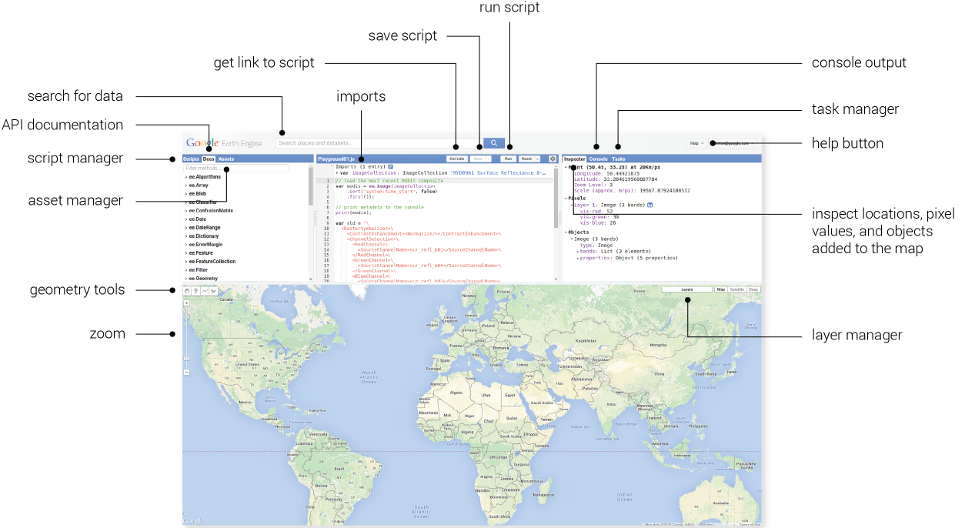
\includegraphics{index_files/mediabag/annotated_playground.png}

(Source: Google Earth Engine)

\hypertarget{application-2}{%
\section{Application}\label{application-2}}

\begin{itemize}
\tightlist
\item
  This is a summary of the applications of GEE
  \includegraphics{index_files/mediabag/amani7-3021052-small.gif}

  (Source: M. Amani et al., 2020)
\end{itemize}

\bookmarksetup{startatroot}

\hypertarget{section}{%
\chapter{}\label{section}}

\href{/data/Monitoring_inland_water_bodies.gif}{11}

\bookmarksetup{startatroot}

\hypertarget{section-1}{%
\chapter{}\label{section-1}}

1

\bookmarksetup{startatroot}

\hypertarget{references}{%
\chapter*{References}\label{references}}
\addcontentsline{toc}{chapter}{References}

\markboth{References}{References}

\hypertarget{refs}{}
\begin{CSLReferences}{1}{0}
\leavevmode\vadjust pre{\hypertarget{ref-knuth84}{}}%
Knuth, Donald E. 1984. {``Literate Programming.''} \emph{Comput. J.} 27
(2): 97--111. \url{https://doi.org/10.1093/comjnl/27.2.97}.

\end{CSLReferences}



\end{document}
